\documentclass[margin,line]{resume}
\usepackage[utf8]{inputenc}
\usepackage[T1]{fontenc}
\usepackage{graphicx}
\usepackage[]{multirow}
\usepackage{hyperref}
\begin{document}

\hfill
\begin{tabular}{r r}
  Laajavuorentie 9 b 25 & \multirow{6}{*} {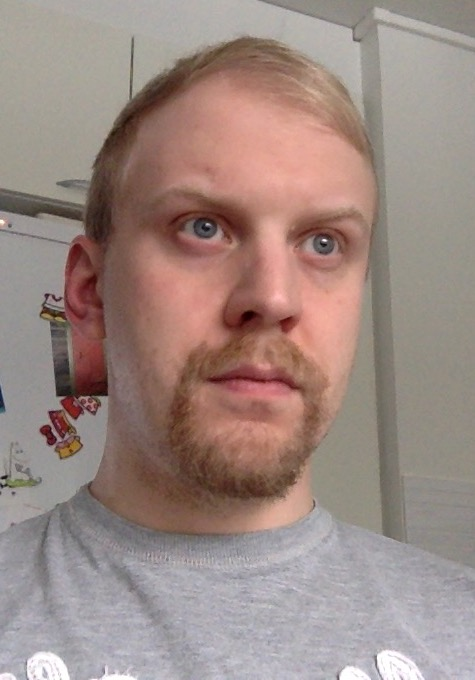
\includegraphics[scale=0.1]{larvi}} \\
  40740 Jyväskylä & \\
  +358415072725 & \\
  tsoikkeli@gmail.com & \\
  http://t-m.fi & \\
  @tusoikke &
\end{tabular}

\vspace{0.5cm}

\name{\Large Tuomas-Matti Soikkeli}
\begin{resume}

\vspace{0.5cm}

\section{\mysidestyle Summary}
I am an information technology enthusiast. I'm an avid programmer with interests in user experience, cloud computing and web development. My most prominent skillset revolves around JavaEE and web applications. In my spare time I like to spend time with my two lovely children. I also enjoy music and gaming in their diverse forms.

\section{\mysidestyle Professional\\Experience}

\textbf{Software Developer}, \href{http://www.descom.fi}{Descom Oy}
\hfill\textbf{Spring 2014}\\
Hardcore enterprise software development in logistics domain using Agile, Scrum, JavaEE, Hibernate, Knockout.js, jQuery, REST, SOAP, Git, Maven, Vagrant, Docker, Microservices, Netflix OSS, Spring Boot, Jenkins and Jira.

\textbf{Software Developer, Architect, Consultant}, Droidoro Oü
\hfill\textbf{2013--}\\
Mobile software design and implementation including low-level communications protocol implementation. Backend service development with Spring stack.


\textbf{Teaching Assistant}, University of Jyväskylä  
\hfill\textbf{Spring semester 2014} \\
Teaching assistant in Basic Game Programming course using C\#/XNA

\textbf{Software Developer}, kateiskuitti.fi
\hfill\textbf{January 2014} \\
Designed and programmed receipt printer desktop software using Java with Swing.

\textbf{Software Specialist}, City of Jyväskylä
\hfill\textbf{September 2012 -- September 2013}\\
Superuser, trainer and application specialist in Effica (healthcare and patient records management software) by Tieto corporation.

\textbf{Backend Programmer}, University of Jyväskylä 
\hfill\textbf{Winter semester 2012}\\
Backend programmer in a student project between Tieto corporation and University of Jyväskylä. I designed and programmed RESTful web service using Java, MongoDB, JAX-RS technology stack.
    
\textbf{Teaching Assistant}, University of Jyväskylä  
\hfill\textbf{Spring semester 2012}\\
Teaching assistant in Programming 1 course. I taught basic programming skills with Java language throughout the course.

\textbf{Web Developer}, Freelancer
\hfill\textbf{2003}\\
Crafted a static website from graphical layouts using HTML and CSS.

\section{\mysidestyle Education}

\textbf{University of Jyväskylä}, Information Systems Science \hfill \textbf{2009--} \\
Bachelor of Science (Economics) Student \\
Thesis: NoSQL-databases: comparsion to relational databases and classification by data model.

\textbf{College of Jyväskylä} \hfill \textbf{ 2006--2009}\\
\textsl{Practical Nurse} 

\textbf{Rudolf Steiner School of Jyväskylä} \hfill \textbf{1994--2004}\\
\textsl{Undergraduate} 

\section{\mysidestyle Other work experience}
\textbf{Supervisor for Mentally Handicapped}, City of Jyväskylä \hfill\textbf{2007--2013}\\
\textbf{Psychriatric Nurse}, Central Finland Health Care District
\hfill\textbf{2010-2011}\\
\textbf{Shift Manager}, Hesburger Oy \hfill\textbf{2006-2009}\\
\textbf{Ranger}, Conscription (6 months) \hfill\textbf{2004-2005} 
\pagebreak 
  
\section{\mysidestyle Language Proficiency}
Finnish: Native language \\ 
English: Excellent written and comprehended, good oral \\ 
Swedish: Basics \\ 
German: Basics 

\section{\mysidestyle Certificates, Licenses} 
AngularJS Advanced training, Profit Oy, 2015 \\
Drivers licence (ABC) \\
First aid licence (2008) \\
Hygiene licence (2004) \\

\end{resume}
\end{document}
